\documentclass{thesisreport}
\usepackage{todonotes}
\usepackage{parskip}
\usepackage{graphicx}
\usepackage{float}
\usepackage{multicol} %aggiunto da me
\usepackage{enumitem}
\usepackage{caption}

\documentclass[main.tex]{subfiles}
\begin{document}
\begin{center}
\begin{longtable}{ |p{0.8cm}p{6.8cm}|p{0.8cm}p{6.8cm}|  }
 \hline
 \multicolumn{4}{|c|}{Instrumental ADL} \\
 \hline
 \textit{\textbf{Score}} & \textit{\textbf{Activities}} & \textit{\textbf{Score}} & \textit{\textbf{Activities}}\\
 \hline
 \vspace{0.15cm} & & &\\
 
  & \textbf{A. Ability to use telephone}  & & \textbf{E. Laundry}  \\
  
 1 & A.1 Operates telephone on own initiative; looks up and dials numbers, etc. & 1  & E.1 Does personal laundry completely \\
 
 1 & A.2 Dials a few well-known numbers & 0 &  E.2 Launders small items; rinses stockings, etc.\\
 
 1    & A.3 Answers telephone but does not dial & 0 & E.3 All laundry must be done by others.\\
 
 0 & A.4 Does not use telephone at all. & & \\
 
 \vspace{0.15cm} & & &\\

 & \textbf{B. Shopping} & & \textbf{F. Mode of Transportation} \\
 
 1 & B.1 Takes care of all shopping needs independently & 1 & F.1 Travels independently on public transportation or drives own cars. \\
 
 0 & B.2 Shops independently for small purchases & 1 & F.2 Arrange own travel via taxi, but does not otherwise use public transportation.\\
 
 0 & B.3 Needs to be accompanied on any shopping trip. & 1 & F.3 Travels on public transportation when accompanied by another.\\
 
 0 & B.4 Completely unable to shop. & 0 & F.4 Travel limited to taxi or automobile with  assistance of another.\\
 
 & & 0 & F.5 Does not travel at all.\\
 
 \vspace{0.15cm} & & &\\

 & \textbf{C. Food Preparation} & & \textbf{G. Responsibility for own medications}\\
 
 1 & C.1 Plans, prepares and serves adequate meals independently & 1 & G.1 Is responsible for taking medication in correct dosages at correct time.\\
 
 0 & C.2 Prepares adequate meals if supplied with ingredients & 0 & G.2 Takes responsibility if medication is prepared in advance in separate dosage.\\
 
 0 & C.3 Heats, serves and prepares meals or prepares meals but does not maintain adequate diet. & 0 & G.3 Is not capable of dispensing own medication.\\
 
 0 & C.4 Needs to have meals prepared and served. & & \\
 
 \vspace{0.15cm} & & &\\
  
 & \textbf{D. Housekeeping} & & \textbf{H. Ability to Handle Finances}\\ 
 
 1 & D.1 Maintains house alone or with occasional assistance (e.g. “heavy work domestic help”) & 1 & H.1 Manages financial matters independently (budgets, writes checks, pays rent, bills goes to bank), collects and keeps track of income.\\
 
 1 & D.2 Performs light daily tasks such as dish-washing, bed making & 1 & H.2 Manages day-to-day purchases, but needs
help with banking, major purchases, etc.\\

 1 & D.3 Performs light daily tasks but cannot maintain acceptable level of cleanliness. & 0 & H.3 Incapable if handling money.\\
 
 1 & D.4 Needs help with all home maintenance tasks. & & \\
 0 & D.5 Does not participate in any housekeeping tasks. & &\\
  
 \hline
\end{longtable}
\captionof{table}{Instrumental Activities of Daily Living Scale \cite{lawton1970assessment}.}
\label{tab:IADL}

\end{center}
\end{document}

\begin{document}

\thispagestyle{empty}

\def\lskip{\vspace{0.5cm}}


\begin{tabular}{p{7cm}p{10cm}}
ÉCOLE CENTRALE DE NANTES
&
\raggedleft UNIVERSITÀ DEGLI STUDI DI GENOVA	% for EMARO students
\end{tabular}

\vspace{2cm}

% EMARO students
\begin{center} \large\sc MASTER ERASMUS MUNDUS \\ \normalsize{EMARO+ ``European Master in Advanced Robotics''} \end{center}


\begin{center}
	2018 / 2019\\
	\lskip
	Master Thesis Report
	\lskip
	
	Presented by \lskip 
	
	Tommaso Elia \lskip
	
	28/12/2018 \lskip\lskip
	
	{\Large \textbf{Dialogue-based interaction processes with smart homes and companion robots}}
	
	\vfill

Jury \lskip
		
	\end{center}
	


\begin{tabular}{p{3cm}p{6cm}p{6cm} }
 President: & Name & Position (Institution) \\ & & \\ 
 Evaluators: & Name & Position (Institution) \\
	      & Name & Position (Institution) \\ 
	      & Name & Position (Institution) \\ & & \\  & & \\ 
  Supervisor(s):  & Fulvio Mastrogiovanni & Assistant Professor (UNIGE)\\
		  & Enrico Reboscio & Project Menager (DotVocal S.r.l.) \\
		  & Renato Zaccaria & Assistant Professor (UNIGE) \\
(EMARO)  & Co-supervisor from M1 & Position, M1 institution 
\end{tabular}

\lskip

\begin{flushleft}
 Laboratory: Laboratoire des Sciences du Numérique de Nantes LS2N
\end{flushleft}

\newpage
\thispagestyle{empty}
\null
\newpage
\addtocounter{page}{-1}
\pagestyle{fancy}
  
 
\section*{Abstract}
   
 Do not forget to check each reference while importing in your Bibtex file.
 Especially, IEEExplore export may lead to ill-formatted conference name like \emph{Robotics and Automation, 
 IEEE International Conference on}.
 
 \newpage
 
 %\section*{Acknowledgements}
 %\newpage
 
\section*{Notations}
 
 \newpage
 
 \section*{Abbreviation}
 
 \begin{tabular}{p{2cm}p{12cm}}
 ADL & Activities of Daily Living\\
 AAL & Ambient Assisted Living \\
 IADL & Instrumental Activities of Daily Living \\
 DS & Dempster - Shafer \\
 DL & Description Logic \\
 SWRL & Semantic Web Rule Language\\
 OWL & Ontology Web Language\\
 EMS & Emergency Medical Services \\
 AR & Activity Recognition \\
 IOT & Internet of Things \\
 ML & Machine Learning \\
 TBox & Terminological Box \\
 ABox & Assertional Box \\
 \end{tabular}
 
 \newpage
 
 \listoffigures
 
 \listoftables
 
 \tableofcontents
 
 
 \chapter{Introduction}
 \addcontentsline{toc}{chapter}{Introduction}	 % non-numbered chapters do not appear in table of contents by default

\section{Motivation}
  The demographic growth along with progress of medical technologies results in an increase of elderly population. Indeed in most of the industrialized countries the demographic and social trends have led to greater elderly burden among the population, and that situation critically increases health care demand. Therefore, emergency medical services, public and private health care and patients are subject to more and more stress. 
  In particular, the raising of the average age of the population means higher incidence of chronic diseases that require frequent health assistance can result in disability and/or lost of independence and deaply affect health economy for the increasing cost of care. Moreover, if there is a suboptimal management of these diseases there is also in increase use of Emergency Medical Service (EMS), often avoiable.
 
 In the district of Kaiserslautern, Germany, a significant study was conducted showing that 44\% of Emergency Medical Services (EMS) are dedicated to elderly above 70 years of age \cite{kleinberger2007ambient}.
 	\begin{figure}[H]
		\centering
		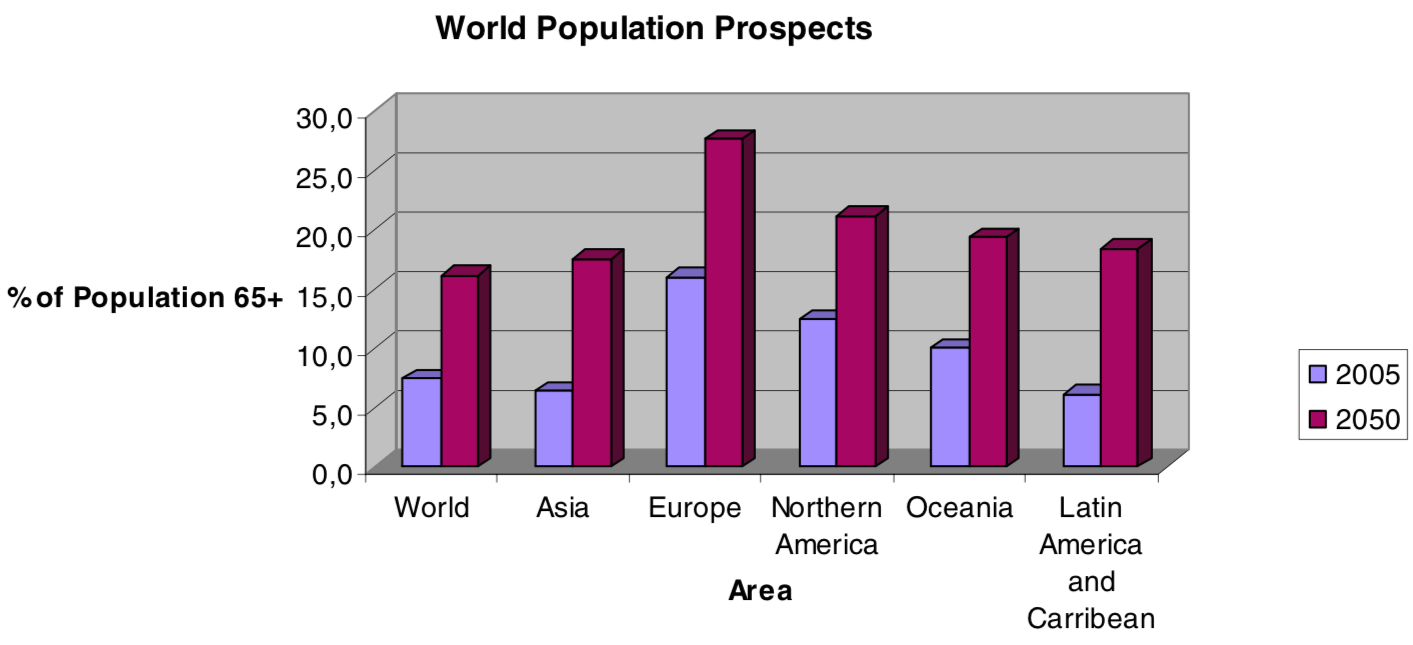
\includegraphics[width=15cm]{Thesis/data/populationProspect.png}
		\caption{\small{Demographical Change according to the United Nations World Population Prospects \cite{kleinberger2007ambient}}}
		\label{fig:populationProspect}
	\end{figure}
 All these elements highlight the increase cost of health care, the underperforming management of resources and the decline of service quality.
 
 \parskip  \parskip
 
 The Ambient Intelligence technologies help to cope with trends, providing proactive and conscious assistance and supporting the autonomy of the elderly, indeed Assisted Living solutions not only can reduce the costs of managing and monitoring older people but can also offer better \textit{quality of life} \cite{kleinberger2007ambient}.
 
 
 \section{Context of the Study}
  To guarantee an improved quality of life it is necessary ensure that the Activities of Daily Living (ADL) are correctly and regularly performed by the assisted \cite{buoncompagni2017towards}.
 
 ADL are defined as daily activities related to motion, rest, nutrition, and personal hygiene, which are a qualitative indicator of person’s wellbeing, determining their quality of life and level of independence \cite{buoncompagni2017towards}. 
 
 At this pourpose, in literature the term smart home is used as synonymous of a home based that is context-aware, context awareness has been defined as: ”having information that can be used to characterize the situation of an entity, where an entity can be a person, place, physical or computational object that is considered relevant to the interaction between a user and an application, including the user and applications themselves” \cite{abowd1999towards}. 

 Today, the idea of smart home is deeply changed, especially due to giant stride of the technologies that support it, giving the possibility to create increasingly complex and sophisticated architectures of intelligent environments. At this regard, in the domain of assistive robots and IOT (Internet of Things) field has taken a leading role, also for technological advances in the miniaturization and increased battery life of different types of sensors \cite{phdthesis} \cite{nakashima2009handbook}.
 
 For an easier and immediate comprehension of the possibilities practicable by this type of technology let's have look to some interesting scenario that could support elderly to retrieve their independence:
 \begin{itemize}
     \item \textit{Scenario 1}: The geriatrician with the task of monitoring the health status of elderly could monitor the quality of the patient's sleep through indomitable devices or pressure sensors positioned at the base of the bed, visualizing the pattern of sleep during the night.
     \item \textit{Scenario 2}: The system could monitor the daily activities such as getting out of bed, washing and having breakfast etc. and if the patient, for example, stop eating the system advises the geriatrician.
     \item \textit{Scenario 3}: The elder after having woken up decides to take a walk, he puts on his coat and as soon as he crosses the threshold the system realizes that it is probable that it rains and that the elder has not taken the umbrella risking thus to fall ill. Then the system alerts him via a notification on the wearable device or directly via a voice interface.
     \item \textit{Scenario 4}: The elderly person who is alone at home  and is heading to the bathroom to wash. The system detects his presence in the bathroom and also receives an unclear signal from the wearable that he wears that could represent a fall by the elderly. To be certain of the elderly safety, the system could verify it  in two ways: it could ask the elderly about his state through a voice interface or it could send a robot 'companion' to check the situation (for example through image analysis - ML).
 \end{itemize}
 
 Smart systems are an very usefull reality but it is important to don't forget to neglect the value of human-human interaction because we do not want that the elderly, that are already at risk of isolation, inserted in this context, isolates himself from the others more than before after being insert in this contest \cite{phdthesis}.
 
 \section{Objectives}
 There are many difficulties and challenges in the smart environment, many of them linked to the importance of the general acceptance of the system by the elderly, allowing them to learn how to get used to the assistance provided. For this reason, the system must meet the following user interface requirements:
 \begin{itemize}
     \item Adaptability:  the systems need to adapt themselves to the context at runtime.
     In order to guarantee the best possible service, the system adapts themselves according to the situation in which they are located, for example reducing the complexity of the interface in case of emergencies to reduce the cognitive load.
     To do this, the system must be able to monitor the environment around it at all times, to reason on what it perceives and then make the necessary adjustments.
     \item  Natural, anticipatory human-computer interaction: the system must provide different levels of interfaces for different types of users; in particular for the medical and assistance staff, for the operators of the maneuvering but especially for the assisted persons whose interface must be specially designed according to the their limitations. 
     Indeed the anticipatory interfaces that proactively contact persons in certain situations are considered mandatory.
     \item Heterogeneity: the system must be able to integrate different subsystems supplied by different manufacturers, providing a unique and homogeneous user interface.
 \end{itemize}
 At the same time, however, we need to consider the medical, technological, social constraints and their consequent problems, for example the difficulties for an elderly person to adapt and understand a new technology, or the difficulties of a system to be operative from the beginning.
 
 Given the complexity of the architecture and of the issues in ambient intelligence, the aim of this thesis work is, firstly, studing and using an already pre-existing architecture, examinig its dinamics, characteristics and the underling strengts and weakness. Secondly, this study’s aim is to improve the architecture ability to acquire informations also in an equivocal and ambiguous context.
 
 The architecture chosen is called Arianna+ and was developed by Teseo Srl in collaboration with the University of Genova. Arianna+ is a smart home system capable of understanding and making sense of the activities carried out by assisted people, predicting their future behaviours and suggesting personalised healthy habits.
 
 Therefore, in short, the goal is to extend Arianna's AI system as follows:
 \begin{itemize}
     \item Allow Arianna+ to intentionally acquire information when a given context or situation is equivocal, with 2 different approaches:
     \begin{itemize}
         \item integrating of a companion robot with the aim of using sensory information collected by robot-centered sensors, building a reciprocal communication whereby the   all the data from the robot are provided to Arianna’s AI system and the AI can control the robot;
         \item integrating a Google Speech API based dialogue management system developed by the company Dot Vocal srl, where each dialogue is modulated by Arianna’s AI system; 
     \end{itemize}
 \end{itemize}

 The goal is therefore to fit these characteristics in a smart home able to acquire sensory data and save them neatly relying on the context. As result of this approach, a high-level artificial intelligence is able to react also to unclear and uncertain situation, such as scenario 4, through an accurate activities’ detection from the environment and flexible and effective management of saved informations.
 
 In this way, the outcome will be an improvement of the system not only functionally but also simplifying its interface with the user.
 Indeed, with the integration of a voice interface and a robot companion the user will be encouraged to no longer see the house as a taciturn and hidden entity but as a like-pet to interact with or a person to talk to in case of need and beyond.
 
\section{Overview of the Thesis}
The remainder of the thesis is organized as follows. 

\quad \textit{Chapter 2} presents an overview of the main concepts and techniques adopted in the ambient intelligence field, from the choice of sensors to how and when use them, not forgetting ADL and Ontology definitions that are crucial to understand their role in the next chapters

\quad \textit{Chapter 3} presents the state of the art regarding the topics that are useful to reach our goals:
\begin{itemize}
    \item Section \ref{Arianna}: presents software architecture of Arianna+ and describes the operating mechanisms to manage data from sensors and to recognize elderly activities.
    \item Section \ref{speech}: presents the state of the art for based dialogue management system in smart environment, in particular the possible approaches and solutions that can be adopted in our case
    \item Section \ref{companionRobot}: presents the state of the art for usage of companion robots in smart environment discussing the advantages and possible choices.
\end{itemize}

 \chapter{Background}
The objective of this chapter is to discuss briefly the different aspects that concern smart environment systems:
\begin{itemize}
    \item The types of sensors that an intelligent box should be equipped with
    \item Possible context models to represent a given context based on sensory information
    \item What are the ADL and how to recognize them
    \item How to guarantee the reliability of the recognition 
\end{itemize}

 \section{Sensoring}
 An architecture able to monitor these kind of activities can provide very useful information about human behaviour to Human-Robot interaction or cooperation in smart environments \cite{bruno2014public}.  
 
 In literature it is possible to distinguish two different approaches of monitoring: one is based on heterogeneous sensor distributed in an area used to deduce the state of the person inside a context \cite{aggarwal2011human}; the other achieves the information from the wearable devices which are sensors located on the person body that are able to detect its movements and vital signs \cite{bao2004activity}. 
 Therefore we can differentiate two different pivotal concepts:
 \begin{itemize}
    \item to monitor complex sequences of activities reported over time and detected by the interaction with various objects in the monitored area, smart environments are the suggested approach \cite{scalmato2012describing}.
    \item with the advent of the Inertial Measurement Unit (IMU) and consequent improvement of measurability of the acceleration and orientation of limbs, the wearable sensing system (fig:\ref{fig:Wearables}), which is also able to monitor bio signals, is certainly the preferred solution to monitor both body gestures and vital signs \cite{bruno2013analysis}.
    
    \begin{figure}
		\centering
		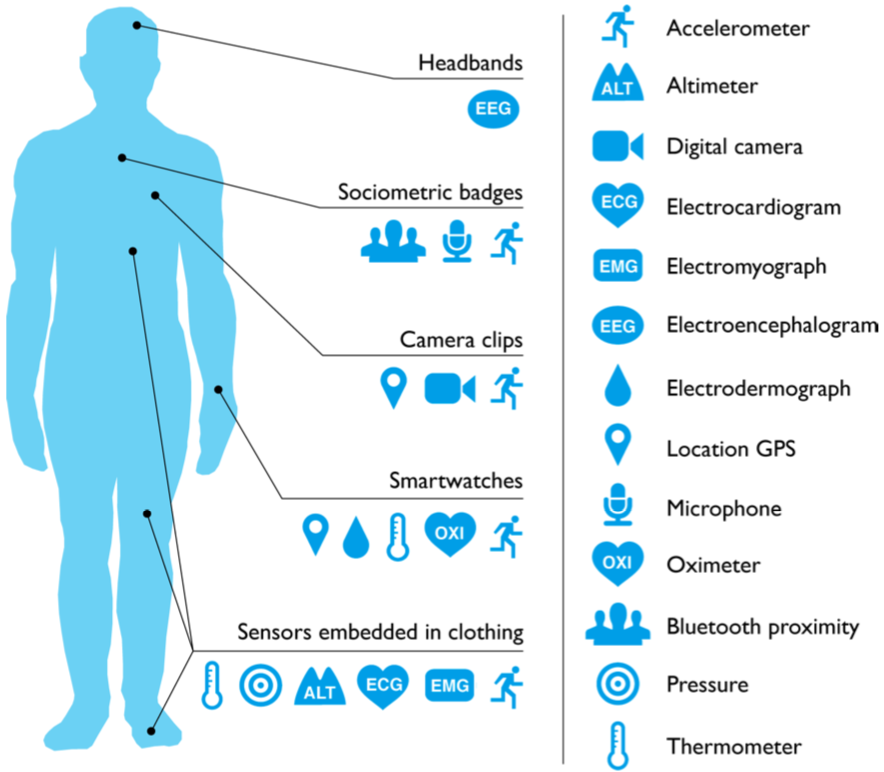
\includegraphics[width=10.5cm]{Thesis/data/sensoring.png}
		\caption{Health Wearables solution \cite{Wearables2016rise}}
		\label{fig:Wearables}
	\end{figure}
    
\end{itemize}
 
 
 
Both these approaches are obviously very useful to detect the state of health of the monitored person and they can be used together because one does not exclude the others. 


\section{Context-Modelling}
 There are several popular context modelling techniques, that are used in context-aware computing. The context models can be either dynamic or static and typically there are two different step that could be distinguished to represent a context according to a model.
 \begin{itemize}
     \item Context modelling process: his function is triggered when a new context need to be defined in terms of characteristics, attributes, relationships with previously specified context, quality-of context attributes and the queries for synchronous context requests.
     \item Organize context according to the model: the result of the context modelling must be validated, then the new context information needs to be merged and added to the existing context information repository and finally make available the new context information when required.
 \end{itemize}
 
 
 \begin{figure}[h]
    \centering
    \begin{subfigure}{0.47\textwidth}
        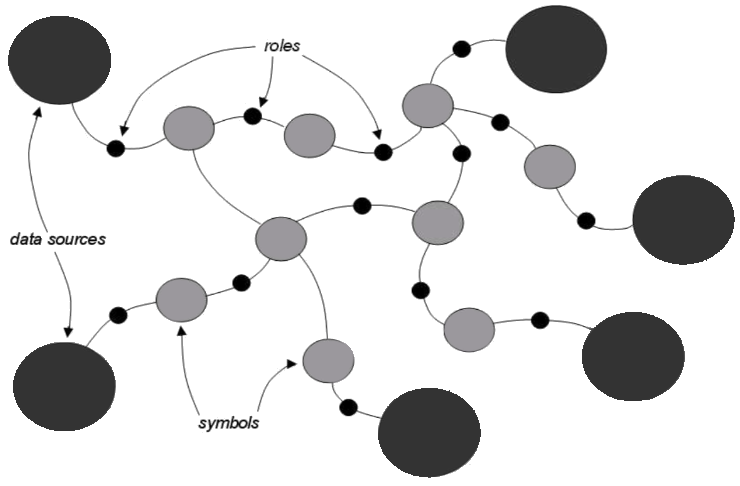
\includegraphics[width=\textwidth]{Thesis/data/ContextModelSketchh.png}
        \caption{A graphical sketch of the\\ proposed context model}
        \label{fig:sketch}
    \end{subfigure}
    \begin{subfigure}{0.47\textwidth}
        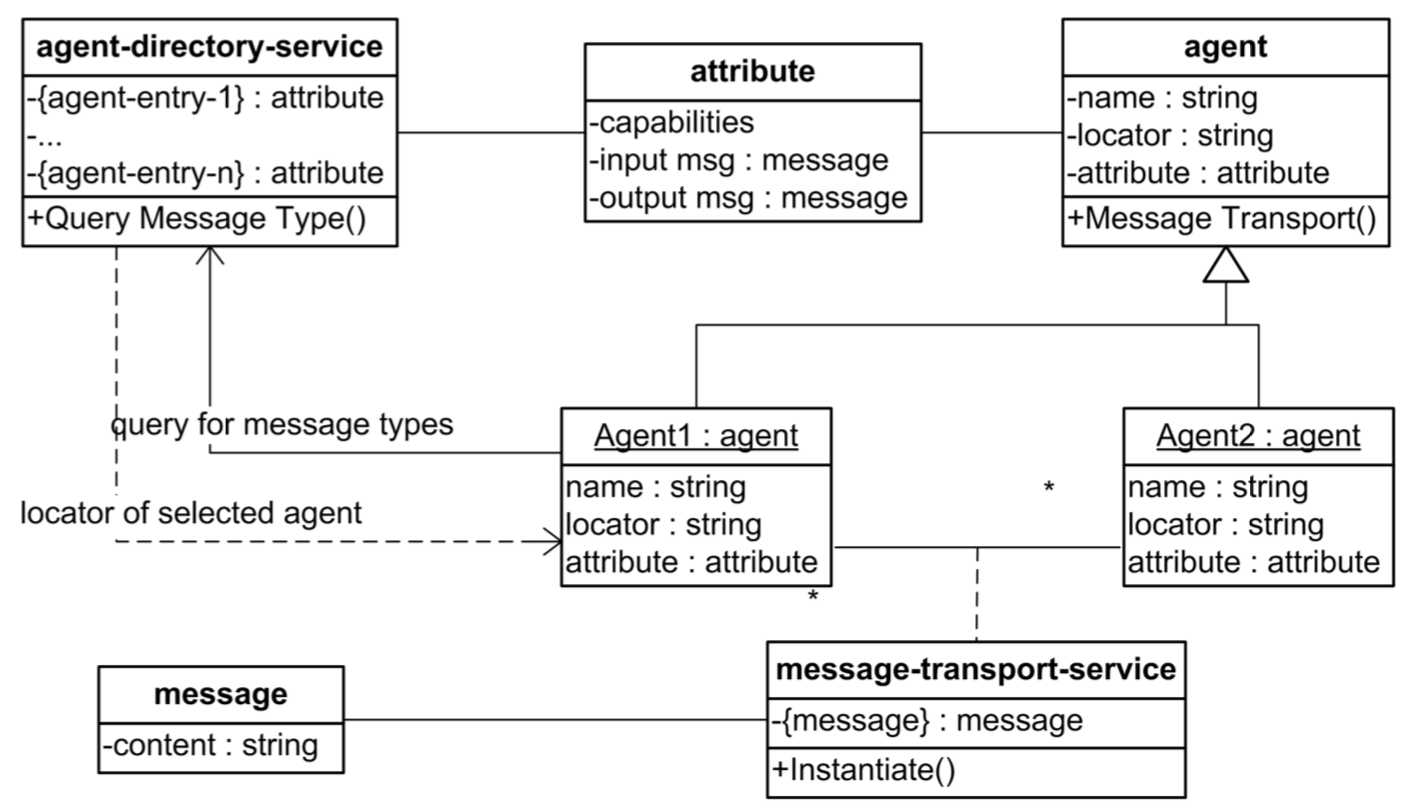
\includegraphics[width=\textwidth]{Thesis/data/architecture.png}
        \caption{A representation of the system architecture.}
        \label{fig:architecture}
    \end{subfigure}
    \caption{Context model sketch and system architecture representation}
    \label{fig:architecture-sketch}
 \end{figure}

 
 However the parameters and factors considered for the modelling context are very subjective. Indeed there is no standard to specify what type information needs to be considered in the context modelling.
 
 Chen at als \cite{chen2000survey} and Strang et als \cite{strang2004context} discussed the most popular context modelling techniques, each of them has its own strengths and weaknesses that are synthetically shown in the table below \cite{perera2014context}.
 
 	\begin{figure}[H]
		\centering
		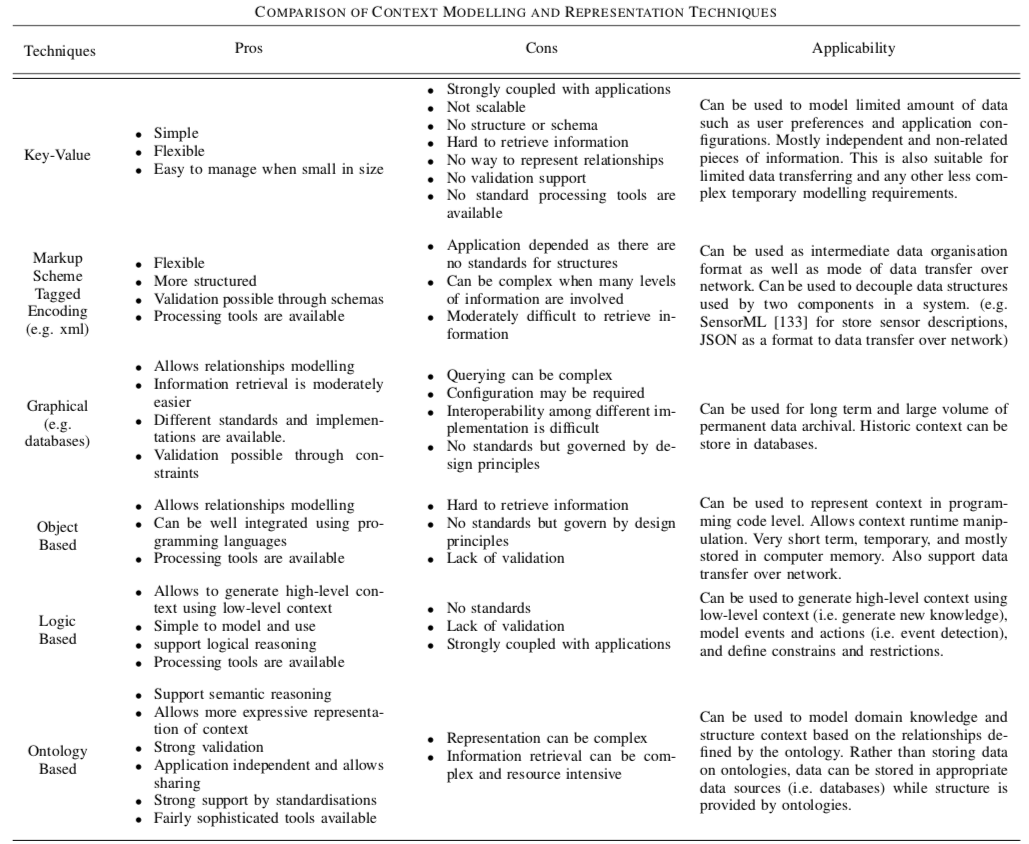
\includegraphics[width=17.5cm]{Thesis/data/ContextModelComparison.png}
		\caption{Comparison of Context Modelling and representation Techniques \cite{perera2014context}}
		\label{fig:populationProspect}
	\end{figure}
 As it will be better discussed in the section \ref{ontology} the ontology, according to many surveys, is the preferred mechanism of managing and and modelling context, for all its advantages and despite its weaknesses \cite{perera2014context}.
 
 
 \subsection{Reasoning}
 The context reasoning, also called inferencing, can be considered as a method to deduct new knowledge based on the available context, indeed it can also be described as a process to provide hight-level context deduction from a set of contexts \cite{perera2014context}.
 There are a lot of context reasoning decision models. Most of these models are not specific to context-reasoning but commonly employed in different fields such as machine learning or artificial intelligence.
 In \textit{"Context aware computing for the internet of things: A survey" Perera et als} \cite{perera2014context} are discussed the main solutions to context-reasoning, here briefly explained: 
 \begin{itemize}
     \item Supervised Learning: in this type of technique first we collect a training set examples. Then we label them according to the results we expect. Then we generate the expected results using the training data.
     They are commonly used where the feature set is easily identifiable.
     
     \textit{Artificial neural network, Bayesian Networks, Case-based reasoning, Decision tree learning, Support vector machines}
     \item Unsupervised Learning: they are used for situations where possible out comes are not known. This type of solution has the great advantage of not needing a training date.
     
     \textit{Clustering, k-Nearest Neighbour}
     \item Rule: applicable for situations where raw data elements need to be converted in to high level context information. Suitable to use to define events , because it needs for few computational resources and storage. Simple to define and easy to extend. 
     \item Fuzzy Logic: applicable for situation where it is necessary convert low-level context in to more high-level context information. It is similar to probabilistic reasoning but confidence values represent degrees of membership rather than probability indeed in traditional logic theory, acceptable truth values are 0 or 1. In fuzzy logic partial truth values are acceptable \cite{perera2014context}. 
     \item Ontology based: It is mainly supported by two common representations of semantic web languages: RDF and OWL. Furthermore, it is based on description logic, which is a family of logic based knowledge representations of formalisms and it is used in case where knowledge is critical and it allows complex reasoning and complex representation basis on the ontology structure.
    
     \textit{First-Order Predicate Logic}
     
     \item Probabilistic logic: it allows decisions relying on probabilities attached to the facts related to the problem. It is commonly used where probabilities are known and combing evidence from different sources are essential. Indeed it can handle unseen situations and of uncertainty, combining the evidence.  
     
     \textit{Dempster-Shafer, hidden Markov Models, naive Bayes}
 \end{itemize}


\section{Ontology} \label{ontology}

\textit{Studer et als} \cite{studer1998knowledge} defines the concept of ontology as follow: 
\begin{center}
\textit{"An ontology is a formal, explicit specification of a shared conceptualisation. A conceptualisation refers to an abstract model of some phenomenon in the world by having identified the relevant concepts of that phenomenon. Explicit means that the type of concepts used, and the constraints on their use are explicitly defined. For example, in medical domains, the concepts are diseases and symptoms, the relations between them are causal and a constraint is that a disease cannot cause itself. Formal refers to the fact that the ontology should be machine readable, which excludes natural language. Shared reflects the notion that an ontology captures consensual knowledge, that is, it is not private to some individual, but accepted by a group.”}
\end{center}


In the ontology based Modelling the context is organized into ontologies with different semantic technologies, indeed there are several popular standards (RDF, RDFS, OWL) and reasonoing capabilities usable depending on the requirement \cite{perera2014context}. 
In literature is clear that the current recommendation, for semantic web ontology, is OWL 2 which is an extended version of OWL \cite{perera2014context}. The strength of OWL2 is that adds more vocabulary for describing properties and classes, ehich could be used to build complex concepts starting with simpler concepts.
Furthermore, to get the real power of semantic technologies we need to choose one reasoning engine and, at this purpose, SWRL is the best  available solutions to add rules in OWL because is fully integrated into ontological reasoning. The dark side of this way of proceeding is that ontologies can becomes exceedingly complex and too much computationally expensive, slowing down the reason process when the amount of data becomes larger and structure becomes too complex.

In conclusion there are several reasons to develop and use ontologies in contrast to other modelling techniques. The most common reasons are:
\begin{itemize}
    \item share a common understanding of the structure of information among people or software agents.
    \item analyse domain knowledge
    \item separate domain knowledge from operational knowledge
    \item high-level knowledge inferring
    \item make domain assumptions explicit
\end{itemize}


\section{ADL}
Our everyday activities tell us a lot about who we are and how ensure a certain level of independence \cite{buoncompagni2017towards}. For this reason at first it is very important to define them. As early as late 1950s, we began the study of psychological, social and biological aspects of aging, analyzing the correlation between human actions and cognitive and motor capabilities \cite{buoncompagni2017towards}. 

The Index of Activities of Daily Living, described in \textit{"Multidisciplinary studies of illness in aged persons"} \cite{Multidisciplinary},  is the most used classification of functional status of elderly people and it is based on their ability to execute six different activities that are defined as ADLs:
%\begin{enumerate}[noitemsep,topsep=1pt,parsep=1pt,partopsep=1pt]
\begin{enumerate}
    \item \textit{bathing}
    \item \textit{dressing}
    \item \textit{toileting}
    \item \textit{transferring}
    \item \textit{continence}
    \item \textit{feeding}
\end{enumerate}

\begin{figure}[H]
	\centering
	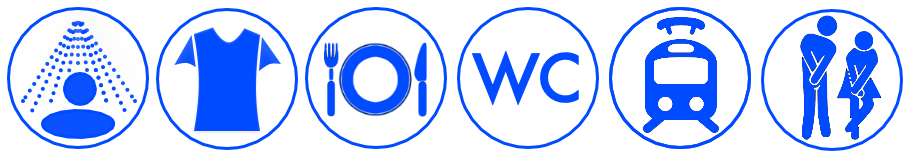
\includegraphics[width=17cm]{Thesis/data/IndexADL.png}
	\caption{Index ADL}
	\label{fig:indexADL}
\end{figure}

But these number of ADL was then extended adding activities deemed relevant for the well-being of a person. These other nine activities, that take the name of Scale of Instrumental ADL \cite{lawton1970assessment} (IADL), require sufficient capabilities of social skills and planning capabilities using and interacting with everyday objects \cite{buoncompagni2017towards}. 
It takes into account 8 parameters, each parameter in turn can have different degrees of autonomy, for each degree of autonomy it is possible to attract the value 1 or the value 0, for a maximum total of 8 points. This concept can be summarized as shown in the table \ref{tab:IADL}. 

\subfile{IADL.tex}

At the end of the evaluation, by performing the sum of the values you can have a score that varies from 0 to 8.

The value 0 represents total dependence, while the opposite is total autonomy.

It is important to remember that if the non-exercise of an activity is not related to a loss of function but to the fact that that activity has never been performed even when the person was healthy and independent, that specific activity should not be considered to calculate the independence of a person.

%\begin{enumerate}[noitemsep,topsep=1pt,parsep=1pt,partopsep=1pt]
% \begin{enumerate}
%     \item \textit{placing a telephone call}
%     \item \textit{shopping}
%     \item \textit{preparing food}
%     \item \textit{housekeeping}
%     \item \textit{doing the laundry}
%     \item \textit{moving outdoor with public transports}
%     \item \textit{moving indoor on foot}
%     \item \textit{taking medications}
%     \item \textit{handling finances}
% \end{enumerate}

Nowadays, as explained in \cite{bruno2014public} the scale of IADL and the index of ADL are the \textit{de facto} standard indexes to evaluate person’s functional status\cite{buoncompagni2017towards}. 

In this essay the term ADL will assume a more general meaning, representing any  considered daily activities. 


\section{Human Activity Recognition}
There are many papers in literature where are discussed the automatic recognition of ADL. There are often differences about adopted sensing equipment or in the choice of the type of sensors, but typically all the solution share a common paradigm: "\textit{distributed sensing, centralized reasoning}". The sensor information are distributed as raw data, with minimal or no processing, and made available to the reasoning system responsible for analyzing them to extract high level information, the ADL \cite{buoncompagni2017towards}.   

A possible solution is to use binary sensors for their easy interpretation (eg: ON/OFF light switch) and their low cost. However, sensory information must be organized and analyzed in higher-level structures and this in literature, the most common and smart solution is doing it with \textit{ontologies}  already discussed in section \ref{ontology} \cite{buoncompagni2017towards}.

\section{Reliability recognition}
The reliability of the recognition is obviously fundamental for any system. Indeed we need to discriminate when a solution is consistent, when all the information is coherent or not with the specific activities detected, when there are some missing information or contradictory.
As explained by \textit{Sentz et als} in \textit{Combination of evidence in Dempster-Shafer theory} \cite{sentz2002combination} to detailed information about the confidence of the recognition, the reasoning module extends a hierarchy of coarse ontologies implementing the Dempster - Shafer (DS). 

However, there are also less extensive solutions, aimed at maximizing the accuracy of the recognition of a single type of ADL. Usually the solutions that follow this paradigm are based on a single or multiple homogeneous sensors that detect the quantities intrinsically correlated to a narrow range of activities. For example, analyzing the flow of water in the house's plumbing system alone can accurately detect when a person is bathing or washing.

 \chapter{State of the art}
 
 \section{Arianna+} \label{Arianna}     \todo{working progress}
 In this section, it is describe a knowledge-based approach for domain modeling (i.e., of context/activity) and reasoning (i.e., context/activity recognition), which is currently part of Arianna+ smart home framework.
 
 
 
 \section{Companion Robot}  \label{companionRobot}
 
 \section{Based dialogue management system} \label{speech}

 %\chapter{Actual work}
  
%  When dealing with rectangled triangles (see Figure \ref{triangle}) I sometimes used this theorem from \cite{pythm001}:
%  \begin{equation}\label{theo}
%   a^2 + b^2 = c^2
%  \end{equation}The demonstration is in Appendix \ref{sec:prooftheorem}.
 
%  \begin{figure}[h]\centering
%   \includegraphics[width=.5\linewidth]{triangle1}
%   \caption{A triangle with letters} \label{triangle}
%  \end{figure}
 
 
%  \chapter{Failed experiments}
 
%  When trying to draw a rectangled triangle, my program comes up with Figure \ref{triangle2} that is neither rectangled nor a triangle.
 
%   \begin{figure}[h]\centering
%   \includegraphics[width=.5\linewidth]{triangle2}
%   \caption{Triangle drawn by my program. Note the 4th side.} \label{triangle2}
%  \end{figure}
 
 
%  \chapter*{Conclusion}
%  \addcontentsline{toc}{chapter}{Conclusion}
 
 
 
%  % switch to A-B-C chaptering
%  \appendix	
 
%  \chapter{Proof of theorem \ref{theo}}
%  \label{sec:prooftheorem}
 
 
%  \begin{proof}
% \eqref{theo} was already demonstrated in \cite{euclides300}.
% \end{proof}
 
 \addcontentsline{toc}{chapter}{Bibliography}

 \bibliographystyle{IEEEtran}
 
 \bibliography{biblio}
 
 
 
 
\end{document}
